% Controller chain v1: how the MACHINE's controller reaches the training loop, and what was
% measured at each step. The evidence companion to closed-loop-form-v4, which argues that the
% residual form is legitimate but says nothing about whether the Cfb inside it is really theirs.
% Written for the ASMPT audience: their doubt is not superposition, it is whether our Python
% controller is their machine's controller.
% Every arrow carries a measured number. A chain without numbers is a flowchart and convinces
% nobody; a chain with a measured error under each link is hard to argue with.
% Vertical, not horizontal: the evidence column needs the width, and five boxes across cannot
% hold the text at a legible size.
% Sources: D-140 (structure + verification), D-099 (aliasing), D-087 (block-mean u), D-141 (4 kHz).
% Style: figure-style.md, notation from the closed-loop table in README.
% Compile: pdflatex controller-chain-v1.tex
\documentclass[border=12pt]{standalone}
\usepackage{tikz}
\usetikzlibrary{arrows.meta, calc}
\usepackage{amsmath}

\begin{document}
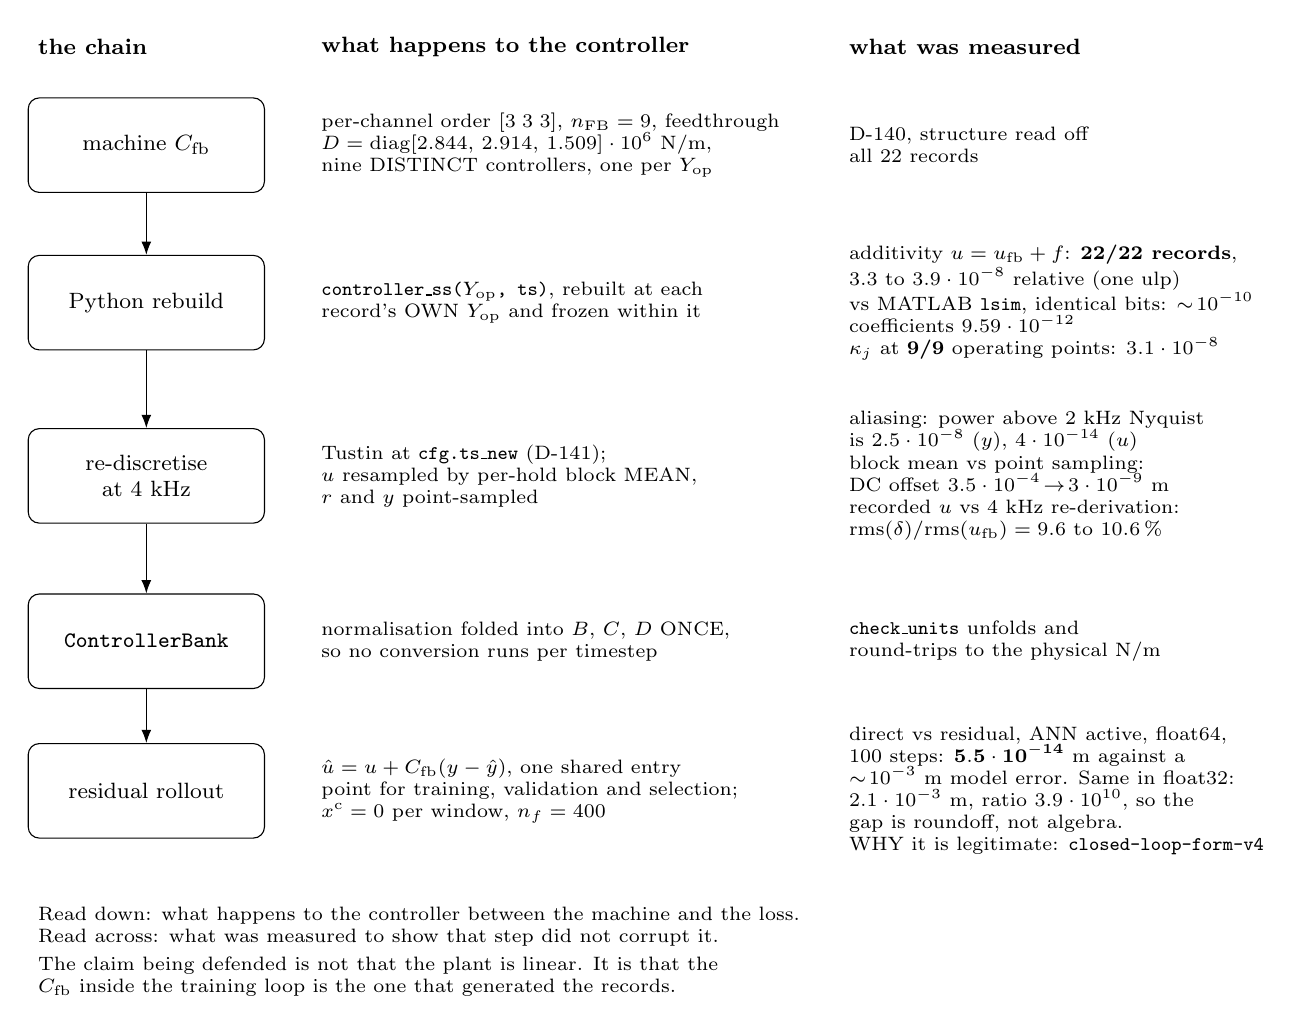
\begin{tikzpicture}[>=Latex, font=\footnotesize,
  block/.style={draw, rounded corners, minimum width=26mm, minimum height=12mm, align=center},
  rblock/.style={draw, rounded corners, minimum width=13mm, minimum height=11mm, align=center},
  small/.style={draw, rounded corners, minimum width=15mm, minimum height=10mm, align=center},
  sum/.style={draw, circle, minimum size=7mm, inner sep=0pt},
  jn/.style={circle, fill, minimum size=3pt, inner sep=0pt}]

\node[anchor=west, font=\footnotesize\bfseries] at (0.10,1.25) {the chain};
\node[anchor=west, font=\footnotesize\bfseries] at (3.70,1.25) {what happens to the controller};
\node[anchor=west, font=\footnotesize\bfseries] at (10.40,1.25) {what was measured};

% ---- 1. the machine ----------------------------------------------------------------
\node[block, minimum width=30mm] (b1) at (1.60,0) {machine $C_{\mathrm{fb}}$};
\node[anchor=west, align=left, font=\scriptsize] at (3.70,0)
  {per-channel order $[3\;3\;3]$, $n_{\mathrm{FB}}=9$, feedthrough\\
   $D=\mathrm{diag}[2.844,\,2.914,\,1.509]\cdot 10^{6}$ N/m,\\
   nine DISTINCT controllers, one per $Y_{\mathrm{op}}$};
\node[anchor=west, align=left, font=\scriptsize] at (10.40,0)
  {D-140, structure read off\\
   all 22 records};

% ---- 2. the rebuild ----------------------------------------------------------------
\node[block, minimum width=30mm] (b2) at (1.60,-2.00) {Python rebuild};
\node[anchor=west, align=left, font=\scriptsize] at (3.70,-2.00)
  {\texttt{controller\_ss($Y_{\mathrm{op}}$, ts)}, rebuilt at each\\
   record's OWN $Y_{\mathrm{op}}$ and frozen within it};
\node[anchor=west, align=left, font=\scriptsize] at (10.40,-2.00)
  {additivity $u=u_{\mathrm{fb}}+f$: \textbf{22/22 records},\\
   $3.3$ to $3.9\cdot10^{-8}$ relative (one ulp)\\
   vs MATLAB \texttt{lsim}, identical bits: $\sim\!10^{-10}$\\
   coefficients $9.59\cdot10^{-12}$\\
   $\kappa_j$ at \textbf{9/9} operating points: $3.1\cdot10^{-8}$};

% ---- 3. the rate -------------------------------------------------------------------
\node[block, minimum width=30mm] (b3) at (1.60,-4.20) {re-discretise\\at 4 kHz};
\node[anchor=west, align=left, font=\scriptsize] at (3.70,-4.20)
  {Tustin at \texttt{cfg.ts\_new} (D-141);\\
   $u$ resampled by per-hold block MEAN,\\
   $r$ and $y$ point-sampled};
\node[anchor=west, align=left, font=\scriptsize] at (10.40,-4.20)
  {aliasing: power above 2 kHz Nyquist\\
   is $2.5\cdot10^{-8}$ ($y$), $4\cdot10^{-14}$ ($u$)\\
   block mean vs point sampling:\\
   DC offset $3.5\cdot10^{-4}\!\rightarrow\!3\cdot10^{-9}$ m\\
   recorded $u$ vs 4 kHz re-derivation:\\
   $\mathrm{rms}(\delta)/\mathrm{rms}(u_{\mathrm{fb}})=9.6$ to $10.6\,\%$};

% ---- 4. the bank -------------------------------------------------------------------
\node[block, minimum width=30mm] (b4) at (1.60,-6.30) {\texttt{ControllerBank}};
\node[anchor=west, align=left, font=\scriptsize] at (3.70,-6.30)
  {normalisation folded into $B$, $C$, $D$ ONCE,\\
   so no conversion runs per timestep};
\node[anchor=west, align=left, font=\scriptsize] at (10.40,-6.30)
  {\texttt{check\_units} unfolds and\\
   round-trips to the physical N/m};

% ---- 5. the rollout ----------------------------------------------------------------
\node[block, minimum width=30mm] (b5) at (1.60,-8.20) {residual rollout};
\node[anchor=west, align=left, font=\scriptsize] at (3.70,-8.20)
  {$\hat u = u + C_{\mathrm{fb}}(y-\hat y)$, one shared entry\\
   point for training, validation and selection;\\
   $x^{\mathrm{c}}=0$ per window, $n_f=400$};
\node[anchor=west, align=left, font=\scriptsize] at (10.40,-8.20)
  {direct vs residual, ANN active, float64,\\
   100 steps: $\mathbf{5.5\cdot10^{-14}}$ m against a\\
   $\sim\!10^{-3}$ m model error. Same in float32:\\
   $2.1\cdot10^{-3}$ m, ratio $3.9\cdot10^{10}$, so the\\
   gap is roundoff, not algebra.\\
   WHY it is legitimate: \texttt{closed-loop-form-v4}};

\draw[->] (b1.south) -- (b2.north);
\draw[->] (b2.south) -- (b3.north);
\draw[->] (b3.south) -- (b4.north);
\draw[->] (b4.south) -- (b5.north);

\node[anchor=north west, align=left, font=\scriptsize] at (0.10,-9.55)
  {Read down: what happens to the controller between the machine and the loss.\\
   Read across: what was measured to show that step did not corrupt it.\\[2pt]
   The claim being defended is not that the plant is linear. It is that the\\
   $C_{\mathrm{fb}}$ inside the training loop is the one that generated the records.};

\end{tikzpicture}
\end{document}
